\documentclass[conference]{IEEEtran}
\IEEEoverridecommandlockouts
\usepackage[utf8]{inputenc}
\usepackage[T1]{fontenc}
\usepackage[spanish]{babel}
\usepackage{amsmath,amssymb,amsfonts}
\usepackage{graphicx}
\usepackage{textcomp}
\usepackage{listings}
\usepackage{xcolor}
\usepackage{float}
\usepackage{booktabs}
\usepackage{cuted}     % entorno strip: bloque a doble columna que no flota
\usepackage{capt-of}   % \captionof, para rotular dentro de un strip
\usepackage{tcolorbox}
\usepackage{eso-pic}
\usepackage{transparent}
\usepackage{hyperref}  % debe cargarse de último para no duplicar anclas de floats

% El informe se compila dentro de reports/entregable1/; las figuras y los
% segmentos de código viven en la raíz del repositorio.
\graphicspath{{../../}}
\newcommand{\repo}{../../}

\pagestyle{plain}

\newif\ifshowwatermark
\showwatermarktrue
\AddToShipoutPictureBG{%
    \ifshowwatermark
        \AtPageCenter{%
            \makebox(0,0){%
                \transparent{0.18}%
                
\includegraphics[width=1.0\textwidth]{assets/images/Logo}%
            }%
        }%
    \fi
}

\lstset{
    language=Python,
    columns=fullflexible,
    basicstyle=\ttfamily\scriptsize\color[RGB]{30,30,30},
    keywordstyle=\bfseries\color[RGB]{0,90,160},
    commentstyle=\itshape\color[RGB]{100,100,100},
    stringstyle=\color[RGB]{160,60,0},
    numberstyle=\tiny\color[RGB]{150,150,150},
    numbers=left,
    numbersep=8pt,
    stepnumber=1,
    backgroundcolor=\color[RGB]{248,248,252},
    frame=none,
    showstringspaces=false,
    breaklines=true,
    breakatwhitespace=false,
    tabsize=4,
    captionpos=b,
    xleftmargin=15pt,
    xrightmargin=5pt,
    inputencoding=utf8,
    extendedchars=true,
    literate=
        {á}{{\'a}}1 {é}{{\'e}}1 {í}{{\'i}}1 {ó}{{\'o}}1 {ú}{{\'u}}1
        {Á}{{\'A}}1 {É}{{\'E}}1 {Í}{{\'I}}1 {Ó}{{\'O}}1 {Ú}{{\'U}}1
        {ñ}{{\~n}}1 {Ñ}{{\~N}}1 {ü}{{\"u}}1 {Ü}{{\"U}}1
        {°}{{\textdegree}}1
        {²}{{$^2$}}1
        {≤}{{$\leq$}}1
        {≥}{{$\geq$}}1
        {→}{{$\rightarrow$}}1
        {·}{{$\cdot$}}1
        {−}{{$-$}}1
        {¨}{}1,
    morekeywords={np, plt, axes, fig, df, pd, sns}
}

\def\BibTeX{{\rm B\kern-.05em{\sc i\kern-.025em b}\kern-.08em T\kern-.1667em\lower.7ex\hbox{E}\kern-.125emX}}

\renewcommand{\refname}{Referencias}

\addto\captionsspanish{%
    \renewcommand{\tablename}{Tabla}%
    \renewcommand{\lstlistingname}{Código}%
}

\begin{document}
    \raggedbottom
    \bstctlcite{IEEEtran:BSTcontrol}

    \title{
        Predicción del puntaje global de la prueba Saber 11 a partir de variables
        socioeconómicas y del colegio: planteamiento del problema y análisis exploratorio
    }

    \author{\IEEEauthorblockN{
        Andrés Giovanny Rubiano Muñoz ``Andy Rubiano''}
        \IEEEauthorblockA{
            \textit{Maestría en Inteligencia Artificial, Facultad de Ingeniería} \\
            \textit{Universidad de La Salle} \\
            Bogotá, Colombia \\
            arubiano67@unisalle.edu.co
        }
    }

    \maketitle
    \thispagestyle{plain}

    \begin{abstract}
    Este informe corresponde a la primera fase del Proyecto Integrador de Ciencia
    de Datos y plantea el problema de predecir el puntaje global de la prueba
    Saber 11 a partir de variables socioeconómicas del hogar, del colegio y del
    estudiante, formulado como una tarea de regresión. Se utiliza el conjunto
    público \textit{Resultados únicos Saber 11} del ICFES, restringido al periodo
    2022-4, descargado desde el Portal Nacional de Datos Abiertos. El análisis
    exploratorio revela que la mitad de las 1.065.888 filas descargadas son
    duplicados exactos, de modo que el conjunto de trabajo queda en 532.792
    estudiantes, y verifica que el puntaje global es una función determinista de
    los puntajes por área, que por tanto se excluyen como variables explicativas.
    La variable objetivo tiene media de 250,1 y desviación de 51,8 puntos, con
    una distribución casi simétrica. Las asociaciones más fuertes corresponden a
    la educación de la madre ($\rho = 0{,}35$), la edad ($\rho = -0{,}32$), la
    educación del padre (0,32) y la tenencia de computador (0,30) e internet
    (0,28); la jornada del colegio separa 70 puntos entre la completa y la
    nocturna, los colegios no oficiales superan a los oficiales en 29 puntos y la
    brecha entre departamentos alcanza 64 puntos entre Bogotá y Chocó. Una
    regresión lineal exploratoria explica el 24,2\,\% de la varianza con un error
    absoluto medio de 36,5 puntos, cota que servirá de referencia para las fases
    de modelado. El informe concluye con doce decisiones de preparación de datos
    e ingeniería de variables derivadas de los hallazgos.
\end{abstract}

\vspace{10pt}

\begin{IEEEkeywords}
    Ciencia de datos, análisis exploratorio de datos, Saber 11, ICFES, regresión,
    datos abiertos, fuga de información, nivel socioeconómico.
\end{IEEEkeywords}


    \section{Introducción}
    La ciencia de datos es la disciplina que combina estadística, computación y
    conocimiento del dominio para extraer, a partir de datos observados,
    conclusiones que respalden decisiones. Un proyecto de ciencia de datos recorre
    un ciclo que comienza con la formulación de una pregunta, continúa con la
    obtención, descripción y exploración de los datos, sigue con la preparación y
    el modelado, y termina con la evaluación y la comunicación de los resultados
    \cite{chapman2000crisp}, \cite{unisalle2026proyecto}. Este informe corresponde
    a la primera fase de ese ciclo, el planteamiento del problema y el análisis
    exploratorio de datos, cuyo propósito es entender la estructura, la calidad y
    las regularidades del conjunto antes de construir cualquier modelo
    \cite{tukey1977exploratory}.

    \vspace{10pt}

    El caso de estudio es la prueba Saber 11, el examen de Estado que presentan en
    Colombia los estudiantes que terminan la educación media y cuyo puntaje global
    condiciona el acceso a la educación superior, a programas de becas y a los
    cupos de las universidades públicas \cite{icfes2022guia}. El Instituto
    Colombiano para la Evaluación de la Educación (ICFES) publica, en el Portal
    Nacional de Datos Abiertos, un registro anónimo por estudiante que reúne el
    resultado de la prueba y un cuestionario sociodemográfico sobre su hogar y su
    colegio \cite{icfes2023resultados}. La literatura sobre los determinantes del
    rendimiento en Saber 11 ha documentado de forma consistente la asociación del
    puntaje con el nivel socioeconómico del hogar, la educación de los padres, la
    naturaleza y la jornada del colegio y la región \cite{gaviria2001determinantes},
    \cite{chica2010determinantes}, lo que convierte al conjunto en un escenario
    adecuado para un problema de aprendizaje supervisado de regresión en el que la
    pregunta no es solo cuánto se puede predecir, sino qué variables, ajenas al
    esfuerzo individual del estudiante, explican esa predicción.

    \vspace{10pt}

    El trabajo se desarrolla en un cuaderno de Google Colab que descarga el
    periodo 2022-4 del conjunto, lo describe, verifica su calidad, caracteriza la
    variable objetivo y examina su relación con las variables del estudiante, del
    hogar, del colegio y de la geografía. Una de las verificaciones es
    metodológicamente central, puesto que el puntaje global se construye como un
    promedio ponderado de los puntajes por área, estos últimos no pueden usarse
    como variables explicativas sin incurrir en una fuga de información
    \cite{kaufman2012leakage}, y el análisis lo comprueba sobre los datos. El
    informe está organizado de la siguiente manera, la Sección~II plantea el
    problema, la pregunta de investigación, los objetivos y las hipótesis; la
    Sección~III describe el conjunto de datos; la Sección~IV expone la metodología
    del análisis exploratorio; la Sección~V presenta los resultados y los primeros
    hallazgos, y la Sección~VI recoge las conclusiones y las decisiones que
    orientan la fase de preparación y modelado.

    \section{Planteamiento del problema}
    Cada año cerca de un millón de estudiantes presentan la prueba Saber 11 en
    el calendario A. El puntaje global que obtienen, en una escala de 0 a 500,
    resume su desempeño en cinco pruebas, lectura crítica, matemáticas,
    competencias sociales y ciudadanas, ciencias naturales e inglés y es el 
    criterio que utilizan las universidades, el programa \textit{Generación E} 
    y otrosmecanismos de acceso a la educación superior \cite{icfes2022guia}.

    \vspace{10pt}
    
    Dado que el ICFES recoge al momento de la inscripción un cuestionario sobre 
    el hogar del estudiante y conoce las características del colegio en el que 
    cursó la media académica, es posible preguntarse en qué medida ese puntaje 
    es predecible a partir de información que existe \textit{antes} de presentar 
    el examen y qué factores pesan más en esa predicción.

    \subsection{Pregunta de investigación}
        ¿En qué medida las características socioeconómicas del hogar, del colegio 
        y aspectos demográficos del estudiante permiten predecir el puntaje global 
        de la prueba Saber 11 y cuáles de esas características tienen mayor peso?

    \subsection{Objetivos}
        \subsubsection{Objetivo general}
            Construir y evaluar un modelo de regresión que prediga el puntaje
            global de la prueba Saber 11 del periodo 2022-4 a partir de variables
            socioeconómicas, familiares y del colegio e interpretar la
            contribución de cada grupo de variables.

            \vspace{10pt}

        \subsubsection{Objetivos específicos}
            \begin{enumerate}
                \item Describir el conjunto de datos \textit{Resultados únicos
                Saber 11} (origen, licencia, variables, tamaño y calidad) y
                caracterizar la distribución de la variable objetivo.

                \item Identificar, mediante análisis exploratorio, las variables
                con mayor asociación con el puntaje global y las que deben
                excluirse por fuga de información o por falta de valor predictivo.

                \item Preparar los datos (tratamiento de valores faltantes,
                codificación de variables ordinales y nominales, ingeniería de
                variables) y establecer un modelo de referencia con su métrica
                inicial.

                \item Entrenar y comparar al menos dos modelos adicionales al de
                referencia, ajustar sus hiperparámetros con validación cruzada y
                evaluarlos con métricas apropiadas para regresión (MAE, RMSE y
                $R^2$).

                \item Interpretar el modelo final (importancia de variables y
                análisis de errores) y comunicar los resultados mediante
                visualizaciones, un informe técnico y una sustentación.
            \end{enumerate}

            Este informe cubre los objetivos específicos 1 y 2, que corresponden
            a la Fase 1 del proyecto, los restantes se abordan en las fases 2, 3 y
            4.

    \subsection{Hipótesis de trabajo}
        \begin{itemize}
            \item \textbf{H1:} El nivel socioeconómico del hogar, medido por el
            estrato, la educación de los padres y el acceso a internet y
            computador es el grupo de variables con mayor asociación con el
            puntaje global.

            \item \textbf{H2:} Las características del colegio, su naturaleza
            oficial o privada, su área urbana o rural, su jornada y su calendario
            aportan información adicional a la del hogar.

            \item \textbf{H3:} Existe una brecha regional, de modo que el
            departamento donde se ubica el colegio explica parte de la variación
            del puntaje incluso después de considerar el hogar y el colegio.
        \end{itemize}

    \subsection{Alcance y restricciones}
        El problema se formula como una regresión sobre el puntaje global. Los
        puntajes por área y el nivel de desempeño en inglés no pueden usarse como
        variables explicativas, porque el puntaje global se calcula a partir de
        ellos y su inclusión constituiría una fuga de información. Se utiliza un 
        único periodo, el 2022-4, para no mezclar escalas ni cuestionarios de 
        distintos años y para mantener el volumen manejable en el entorno gratuito 
        de Google Colab, adicionalmente, se realiza elanálisis es correlacional
        que identifica asociaciones útiles para predecir y no relaciones causales.
    \section{Conjunto de datos}
    \subsection{Origen y licencia}
        El conjunto \textit{Resultados únicos Saber 11} es publicado por el
        Instituto Colombiano para la Evaluación de la Educación (ICFES) en el
        Portal Nacional de Datos Abiertos de Colombia, bajo el identificador
        \texttt{kgxf-xxbe} y con licencia Creative Commons Attribution-ShareAlike
        4.0 (CC BY-SA 4.0), que permite su uso, redistribución y adaptación con
        atribución \cite{icfes2023resultados}. Reúne 7,1 millones de registros
        anónimos de las aplicaciones realizadas entre 2010 y 2022, uno por
        estudiante y periodo, con 51 columnas, y su última actualización data de
        agosto de 2023. El portal expone los datos mediante la API de Socrata, lo
        que permite descargar un periodo específico con un filtro en la URL sin
        necesidad de registro.

    \subsection{Periodo seleccionado y tamaño}
        Se trabaja con el periodo 2022-4, correspondiente a la aplicación del
        calendario A del segundo semestre de 2022, que es la que presenta la gran
        mayoría de colegios del país y el periodo más reciente y numeroso del
        conjunto. La descarga pesa 560 MB y contiene 1.065.888 filas; como se
        muestra en la Sección~V, la mitad de ellas son duplicados exactos y el
        conjunto de trabajo queda en 532.792 estudiantes. La Tabla~\ref{dataset_summary}
        resume sus características.

        \begin{table}[H]
            \centering
            \caption{Resumen del conjunto de datos}
            \label{dataset_summary}
            \begin{tabular}{ll}
                \toprule
                \textbf{Aspecto} & \textbf{Valor} \\
                \midrule
                Fuente & datos.gov.co, conjunto \texttt{kgxf-xxbe} \\
                Publicador & ICFES \\
                Licencia & CC BY-SA 4.0 \\
                Periodo & 2022-4 (calendario A, segundo semestre) \\
                Filas descargadas & 1.065.888 \\
                Filas únicas & 532.792 \\
                Columnas & 51 \\
                Variable objetivo & \texttt{punt\_global} (0 a 500) \\
                Tamaño en disco & 560 MB (CSV) \\
                Tamaño en memoria & 131 MB (tipos categóricos) \\
                \bottomrule
            \end{tabular}
        \end{table}

    \subsection{Variables}
        Las 51 columnas se agrupan en cinco bloques según su prefijo, descritos
        en la Tabla~\ref{variables}. Todas llegan como texto; en el cuaderno las
        categóricas se leen como \texttt{category}, los puntajes como numéricos y
        los identificadores como cadena.

        \begin{table}[H]
            \centering
            \caption{Bloques de variables del conjunto}
            \label{variables}
            \begin{tabular}{p{2.1cm}p{5.6cm}}
                \toprule
                \textbf{Bloque} & \textbf{Contenido} \\
                \midrule
                Identificación (5) & Periodo, identificador anónimo
                (\texttt{estu\_consecutivo}), tipo de documento, condición del
                evaluado y estado del resultado. \\
                Colegio, \texttt{cole\_*} (17) & Códigos DANE e ICFES, nombres
                del establecimiento y la sede, naturaleza (oficial o no oficial),
                área (urbana o rural), calendario, carácter (académico o técnico),
                jornada, género de la población, bilingüismo y ubicación
                (departamento y municipio). \\
                Estudiante, \texttt{estu\_*} (13) & Género, fecha de nacimiento,
                nacionalidad, lugar de residencia, lugar de presentación de la
                prueba y privación de la libertad. \\
                Hogar, \texttt{fami\_*} (9) & Estrato de la vivienda, máximo
                nivel educativo de la madre y del padre, personas y cuartos del
                hogar y tenencia de internet, computador, automóvil y lavadora;
                provienen del cuestionario que el estudiante diligencia al
                inscribirse. \\
                Resultados (7) & Puntaje en lectura crítica, matemáticas,
                sociales y ciudadanas, ciencias naturales e inglés (0 a 100),
                nivel de desempeño en inglés y puntaje global (0 a 500). \\
                \bottomrule
            \end{tabular}
        \end{table}

        La variable objetivo es el puntaje global. Las variables explicativas
        candidatas son las de los bloques de estudiante, hogar y colegio, más el
        departamento y el municipio del colegio; los resultados por área se
        excluyen por la razón que se verifica en la Sección~V.

    \section{Metodología}
    El análisis se realizó en un cuaderno de Google Colab cuyos segmentos de
    código se reproducen a lo largo de este informe en el mismo orden en que se
    ejecutan, puesto que cada paso depende del anterior, iniciando con la
    preparación del entorno, siguiendo con la descarga y verificación del
    conjunto, la depuración de duplicados, el tratamiento de los valores faltantes
    y la conversión de tipos, la caracterización de la variable objetivo y, por
    último, el examen de su relación con cada grupo de variables explicativas. El
    enfoque sigue la lógica del análisis exploratorio de datos de Tukey, mirar los
    datos antes de modelarlos para descubrir su estructura y sus anomalías
    \cite{tukey1977exploratory}, dentro del marco de fases de CRISP-DM
    \cite{chapman2000crisp}.

    \subsection{Entorno de trabajo y reproducibilidad}
        El cuaderno utiliza únicamente librerías preinstaladas en Colab,
        \textit{kagglehub} para descargar el conjunto de datos,
        \textit{pandas} para la carga y agregación de datos
        \cite{mckinney2010pandas}, \textit{matplotlib} y \textit{seaborn} para las
        figuras \cite{hunter2007matplotlib}, \cite{waskom2021seaborn},
        \textit{scipy} para la correlación de Spearman y \textit{scikit-learn} para
        el ajuste lineal exploratorio \cite{pedregosa2011scikit}. Las rutas se
        resuelven respecto de la raíz del repositorio, de modo que las figuras se
        guardan en \texttt{assets/images/data/}, que es de donde las toma este
        informe.

        \vspace{10pt}

        \lstinputlisting{\repo utils/codes/environment-setup/environment-setup.py}

        \vspace{10pt}

        Luego se fija la identidad gráfica, un azul para la variable objetivo y
        las series principales, un naranja para contrastes y un tono neutro para
        las descripciones del conjunto, y la semilla global \texttt{RANDOM\_STATE
        = 42}, que gobierna el único muestreo del cuaderno.

        \vspace{10pt}

        \lstinputlisting{\repo utils/codes/graphic-identity/graphic-identity.py}

    \subsection{Descarga y carga del conjunto}
        El periodo 2022-4 se extrajo del Portal Nacional de Datos Abiertos
        mediante su API, con un filtro por periodo y un orden fijo por
        identificador, y se publicó en Kaggle como el dataset \textit{Saber 11
        Colombia - Resultados 2022-4} \cite{rubiano2026kaggle}, con la misma
        licencia y atribución al ICFES. La copia conserva todas las filas y
        columnas tal como las entrega el portal; el único cambio es el formato,
        de CSV (560 MB) a Parquet (31,5 MB), que además guarda el tipo de cada
        columna: las categóricas como \texttt{category}, los puntajes como
        \texttt{float32} y los identificadores como cadena. Publicar una copia
        congelada hace el análisis reproducible aunque el portal actualice sus
        datos, y reduce la carga del cuaderno a unos segundos. La celda descarga
        únicamente el archivo Parquet con \textit{kagglehub}, que no requiere
        cuenta de Kaggle para un dataset público, y lo lee con \textit{pandas}.

        \vspace{10pt}

        \lstinputlisting{\repo utils/codes/dataset-download/dataset-download.py}

        \vspace{10pt}

        La estructura del conjunto se verifica columna por columna, tipo,
        cantidad de valores no nulos, porcentaje de faltantes, cardinalidad y un
        valor de ejemplo, que es la base del diccionario de variables de la
        Sección~III.

        \vspace{10pt}

        \lstinputlisting{\repo utils/codes/dataset-structure/dataset-structure.py}

    \subsection{Calidad de los datos}
        Se cuentan los registros duplicados y se comprueba si el identificador
        \texttt{estu\_consecutivo} es único; los duplicados exactos se eliminan y
        el resto del análisis se realiza sobre el conjunto depurado. Se
        identifican además las columnas constantes y las de muy poca variación,
        que no aportan información a un modelo, y se tabula la cardinalidad de
        cada variable categórica, que determina su codificación en la fase 2.

        \vspace{10pt}

        \lstinputlisting{\repo utils/codes/data-quality/data-quality.py}

        \vspace{10pt}

        Los valores faltantes se cuantifican por columna y se examina si los del
        bloque \texttt{fami\_*} ocurren juntos, lo que indicaría estudiantes que
        no diligenciaron el cuestionario, o de forma independiente; también se
        compara el puntaje de quienes no tienen cuestionario con el del resto,
        para saber si la ausencia es informativa.

        \vspace{10pt}

        \lstinputlisting{\repo utils/codes/missing-values/missing-values.py}

        \vspace{10pt}

        Por último se convierte la fecha de nacimiento en la edad al momento de
        la prueba, tomando como referencia la fecha de aplicación del calendario A
        de 2022, y se fija el orden natural de las variables ordinales (estrato,
        educación de los padres, personas y cuartos del hogar, nivel de inglés),
        que \texttt{category} no conoce por sí misma.

        \vspace{10pt}

        \lstinputlisting{\repo utils/codes/type-conversion/type-conversion.py}

    \subsection{Variable objetivo}
        La distribución de \texttt{punt\_global} se caracteriza con sus
        estadísticas descriptivas, su asimetría y curtosis, un histograma y un
        diagrama de caja. Luego se verifica la fórmula con la que el ICFES
        construye el puntaje global a partir de las cinco pruebas
        \cite{icfes2022guia},
        \begin{equation}
            \label{global_formula}
            \begin{aligned}
                G = \operatorname{round}\Bigl(\tfrac{5}{13}\bigl(
                    & 3\,LC + 3\,MAT \\
                    & + 3\,SOC + 3\,CN + 1\,ING \bigr)\Bigr),
            \end{aligned}
        \end{equation}
        donde $LC$, $MAT$, $SOC$, $CN$ e $ING$ son los puntajes de lectura
        crítica, matemáticas, sociales y ciudadanas, ciencias naturales e inglés.
        Si la fórmula se cumple sobre los datos, los puntajes por área son
        componentes de la respuesta y no variables explicativas, y su inclusión en
        un modelo constituiría una fuga de información \cite{kaufman2012leakage}.

        \vspace{10pt}

        \lstinputlisting{\repo utils/codes/target-distribution/target-distribution.py}

        \vspace{10pt}

        \lstinputlisting{\repo utils/codes/target-formula/target-formula.py}

    \subsection{Análisis bivariado por grupo de variables}
        Para cada variable categórica se calcula el tamaño, la media, la mediana y
        la desviación del puntaje global por categoría, y se grafica con diagramas
        de caja sin valores atípicos, de modo que la comparación entre grupos no
        quede dominada por los extremos. Dos funciones auxiliares,
        \texttt{resumen\_por} y \texttt{caja\_por}, encapsulan ese patrón y se
        reutilizan en las secciones de estudiante, hogar y colegio. La edad se
        agrupa en tramos, porque su relación con el puntaje no tiene por qué ser
        lineal.

        \vspace{10pt}

        \lstinputlisting{\repo utils/codes/student-variables/student-variables.py}

        \vspace{10pt}

        \lstinputlisting{\repo utils/codes/family-variables/family-variables.py}

        \vspace{10pt}

        Para las variables binarias del hogar se compara la media del puntaje
        entre quienes tienen y no tienen cada bien, y se reporta la diferencia en
        puntos.

        \vspace{10pt}

        \lstinputlisting{\repo utils/codes/family-binary/family-binary.py}

        \vspace{10pt}

        \lstinputlisting{\repo utils/codes/school-variables/school-variables.py}

        \vspace{10pt}

        Como naturaleza y área se cruzan (la mayoría de colegios rurales son
        oficiales), se tabula el puntaje medio en las cuatro combinaciones.

        \vspace{10pt}

        \lstinputlisting{\repo utils/codes/school-crosstab/school-crosstab.py}

        \vspace{10pt}

        Para la geografía se calcula el puntaje medio por departamento del
        colegio, se ordena y se contrasta con la media nacional.

        \vspace{10pt}

        \lstinputlisting{\repo utils/codes/geography/geography.py}

    \subsection{Correlaciones y ajuste lineal exploratorio}
        Las variables ordinales se codifican con enteros que respetan su orden,
        estrato de 0 a 6 y nivel educativo de 0 a 9 (las categorías \textit{No
        sabe} y \textit{No Aplica} se tratan como faltantes), las binarias con 0 y
        1, y se calcula la correlación de Spearman \cite{spearman1904proof},
        \begin{equation}
            \label{spearman}
            \rho = 1 - \frac{6 \sum_{i=1}^{n} d_i^2}{n\,(n^2 - 1)},
        \end{equation}
        donde $d_i$ es la diferencia entre los rangos de las dos variables para la
        observación $i$. Se eligió Spearman en lugar de Pearson porque mide
        asociaciones monótonas, no solo lineales, y es apropiada para variables
        ordinales. La matriz incluye los puntajes por área para documentar el
        contraste entre una variable explicativa legítima y una que forma parte de
        la respuesta.

        \vspace{10pt}

        \lstinputlisting{\repo utils/codes/correlations/correlations.py}

        \vspace{10pt}

        Finalmente se ajusta una regresión lineal exploratoria sobre las
        variables codificadas, excluidos los puntajes por área, con una muestra
        aleatoria de 200.000 filas completas y una partición 80/20. No es el
        modelo de referencia de la fase 2, que se construirá con la limpieza
        completa y la partición definitiva, sino una cota rápida de cuánta
        varianza del puntaje explican las variables candidatas en conjunto,
        medida con el coeficiente de determinación $R^2$ y el error absoluto medio
        (MAE).

        \vspace{10pt}

        \lstinputlisting{\repo utils/codes/exploratory-fit/exploratory-fit.py}

    \section{Resultados}
    \subsection{Calidad de los datos}
        La primera verificación resultó decisiva. De las 1.065.888 filas
        descargadas, 533.096 (50,01\,\%) son duplicados exactos y el identificador
        \texttt{estu\_consecutivo} tiene solo 532.792 valores distintos: cada
        registro aparece dos veces en la tabla del portal. Tras eliminar los
        duplicados quedan 532.792 estudiantes con identificador único, cifra
        coherente con la población que presenta la prueba en el calendario A. El
        hallazgo no habría alterado las medias, pero sí todos los conteos y, en
        la fase de modelado, habría colocado el mismo estudiante en entrenamiento
        y en prueba, inflando artificialmente cualquier métrica.

        \vspace{10pt}

        {\sloppy\hbadness=5000
        Dos columnas son constantes (\texttt{periodo} y
        \texttt{estu\_estudiante}) y tres casi constantes,
        \texttt{cole\_calendario} (99,58\,\% A, porque los colegios de calendario
        B presentan en el periodo 2022-1), \texttt{estu\_estadoinvestigacion}
        (99,96\,\%) y \texttt{estu\_privado\_libertad} (99,95\,\%). Los códigos
        y nombres del colegio tienen entre 9.412 y 13.748 niveles y los
        municipios más de 1.000, mientras que el departamento tiene 33.
        \par}

        \vspace{10pt}

        Los valores faltantes (Fig.~\ref{missing_values}) se concentran en
        \texttt{cole\_bilingue} (18,0\,\%) y en el bloque del hogar (4,3 a
        6,7\,\%); los puntajes están completos salvo inglés (0,37\,\%). El
        2,31\,\% de los estudiantes no respondió ninguna pregunta del
        cuestionario, el 10,14\,\% tiene al menos una respuesta faltante y el
        89,86\,\% lo diligenció completo. La ausencia no es aleatoria, puesto que
        quienes no tienen cuestionario promedian 229,1 puntos frente a 250,6 de
        quienes sí lo tienen.

        \begin{figure}[H]
            \centerline{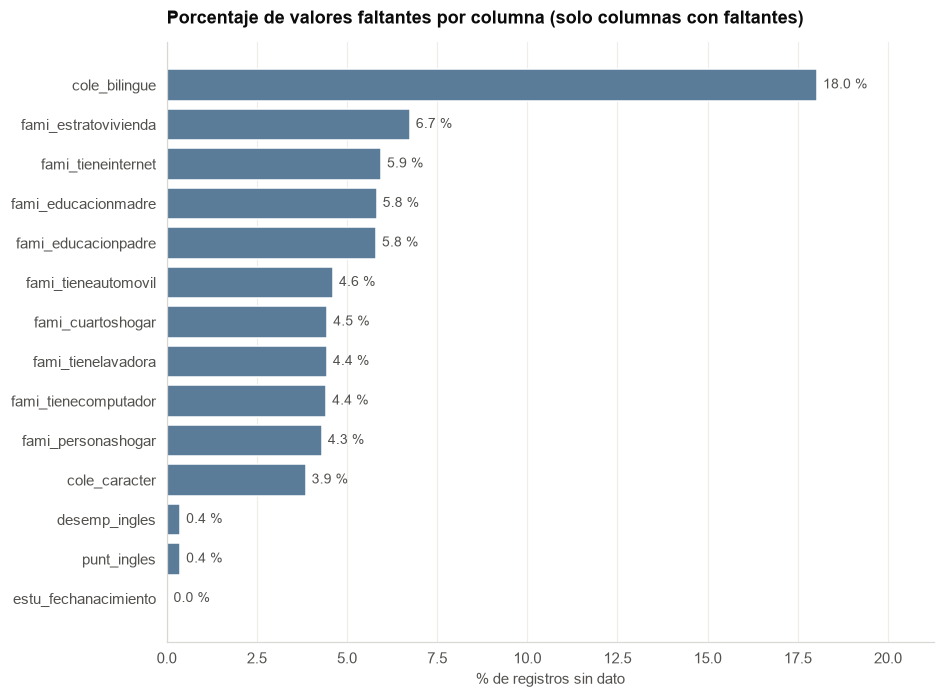
\includegraphics[width=1\linewidth]{assets/images/data/missing_values.png}}
            \caption{Porcentaje de valores faltantes por columna, para las
            columnas que tienen al menos uno.}
            \label{missing_values}
        \end{figure}

        La fecha de nacimiento se convirtió en edad al momento de la prueba, con
        media de 17,8 años, mediana de 17,2 y el 50\,\% central entre 16,7 y 18,1
        años; solo 81 fechas no pudieron interpretarse y 218 edades quedaron
        fuera del rango plausible.

    \subsection{Variable objetivo}
        El puntaje global tiene media de 250,1, mediana de 247 y desviación de
        51,8 puntos; la mitad central de los estudiantes queda entre 210 y 288, el
        1\,\% inferior por debajo de 156 y el 1\,\% superior por encima de 369. La
        asimetría de 0,28 y la curtosis de $-0{,}54$ describen una distribución
        casi simétrica, con una leve cola derecha y colas más ligeras que la
        normal (Fig.~\ref{target_distribution}), de modo que no hace falta
        transformar la variable y las métricas de error se leen directamente en
        puntos.

        \clearpage
        \begin{strip}
            \centering
            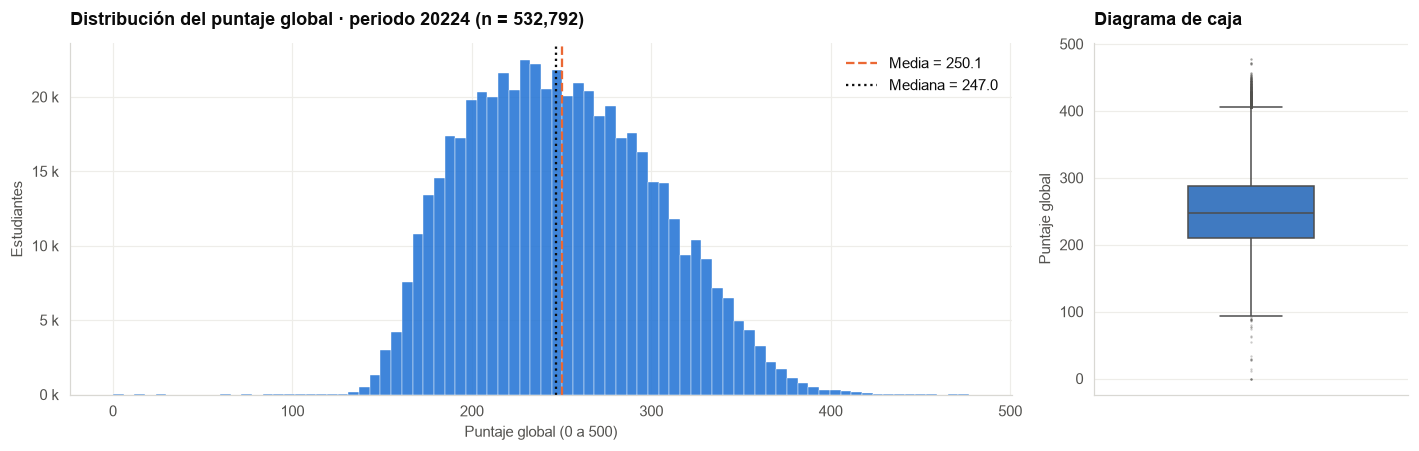
\includegraphics[width=0.98\linewidth]{assets/images/data/target_distribution.png}
            \captionof{figure}{Distribución del puntaje global en el periodo
            2022-4 (532.792 estudiantes): histograma con media y mediana, y
            diagrama de caja.}
            \label{target_distribution}
        \end{strip}

        La fórmula (\ref{global_formula}) se cumple en el 100\,\% de los 530.815
        registros que tienen las cinco pruebas, con una diferencia máxima de cero
        puntos, y cada área correlaciona entre 0,91 y 0,92 con el global (0,80
        inglés). El puntaje global es por tanto una función determinista de los
        puntajes por área, y estos quedan excluidos del conjunto de variables
        explicativas.

    \subsection{Variables del estudiante}
        Los hombres promedian 254,1 puntos y las mujeres 246,8, una brecha de 7,3
        puntos. La edad es una de las variables más informativas
        (Fig.~\ref{student_variables}): los estudiantes de 16 y 17 años promedian
        265 puntos, a los 18 el promedio baja a 250,5, a los 19 y 20 a 229,5,
        entre 21 y 25 a 206,1 y de 26 en adelante a 199,6, una caída de más de 65
        puntos que marca trayectorias de extraedad y educación de adultos. El tipo
        de documento redunda con la edad, la tarjeta de identidad promedia 255,6
        y la cédula de ciudadanía 219,4.

        \begin{strip}
            \centering
            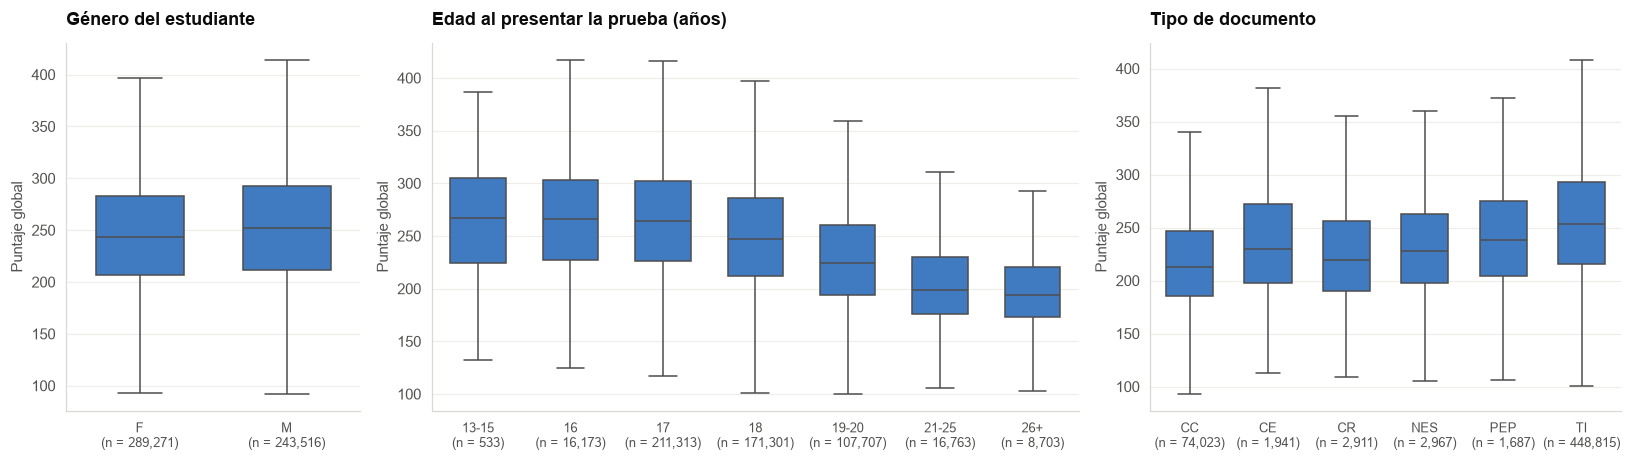
\includegraphics[width=0.98\linewidth]{assets/images/data/student_variables.png}
            \captionof{figure}{Puntaje global según género, tramo de edad y tipo
            de documento del estudiante (diagramas de caja sin valores atípicos;
            $n$ de cada grupo en el eje).}
            \label{student_variables}
        \end{strip}

    \subsection{Variables del hogar}
        La Tabla~\ref{family_table} y la Fig.~\ref{family_ordinal} muestran la
        gradiente socioeconómica. La educación de la madre tiene una relación
        perfectamente monótona con el puntaje, de 211,2 puntos cuando no tiene
        ningún nivel educativo a 307,5 cuando tiene posgrado, 96 puntos de
        diferencia, el contraste más amplio del análisis; la del padre va de 214,5
        a 311,9, y su categoría \textit{No sabe} reúne 36.317 estudiantes
        (6,8\,\%), reflejo de hogares sin presencia paterna, que promedian 260,7.
        El estrato sube de 212,6 (\textit{Sin estrato}) a 267,4 (estrato 4) pero
        cae en los estratos 5 (261,4) y 6 (245,1), que tienen las desviaciones
        más altas y los grupos más pequeños, un quiebre que apunta a errores de
        reporte en el cuestionario.

        \begin{table}[H]
            \centering
            \caption{Puntaje global medio según variables ordinales del hogar}
            \label{family_table}
            \begin{tabular}{|l|r|r|}
                \hline
                \textbf{Variable y nivel} & \textbf{$n$} & \textbf{Media} \\
                \hline
                Estrato: Sin estrato & 19.781 & 212,6 \\
                \hline
                Estrato 1 & 146.333 & 242,0 \\
                \hline
                Estrato 2 & 180.091 & 253,7 \\
                \hline
                Estrato 3 & 110.254 & 263,2 \\
                \hline
                Estrato 4 & 28.092 & 267,4 \\
                \hline
                Estrato 5 & 8.448 & 261,4 \\
                \hline
                Estrato 6 & 3.879 & 245,1 \\
                \hline
                Educ. madre: Ninguno & 10.260 & 211,2 \\
                \hline
                Primaria completa & 42.124 & 233,4 \\
                \hline
                Secundaria completa & 143.736 & 249,4 \\
                \hline
                Técnica o tecnológica completa & 52.289 & 268,0 \\
                \hline
                Educación profesional completa & 62.318 & 278,4 \\
                \hline
                Postgrado & 11.372 & 307,5 \\
                \hline
                No sabe & 12.638 & 261,5 \\
                \hline
            \end{tabular}
        \end{table}

        \clearpage
        \begin{strip}
            \centering
            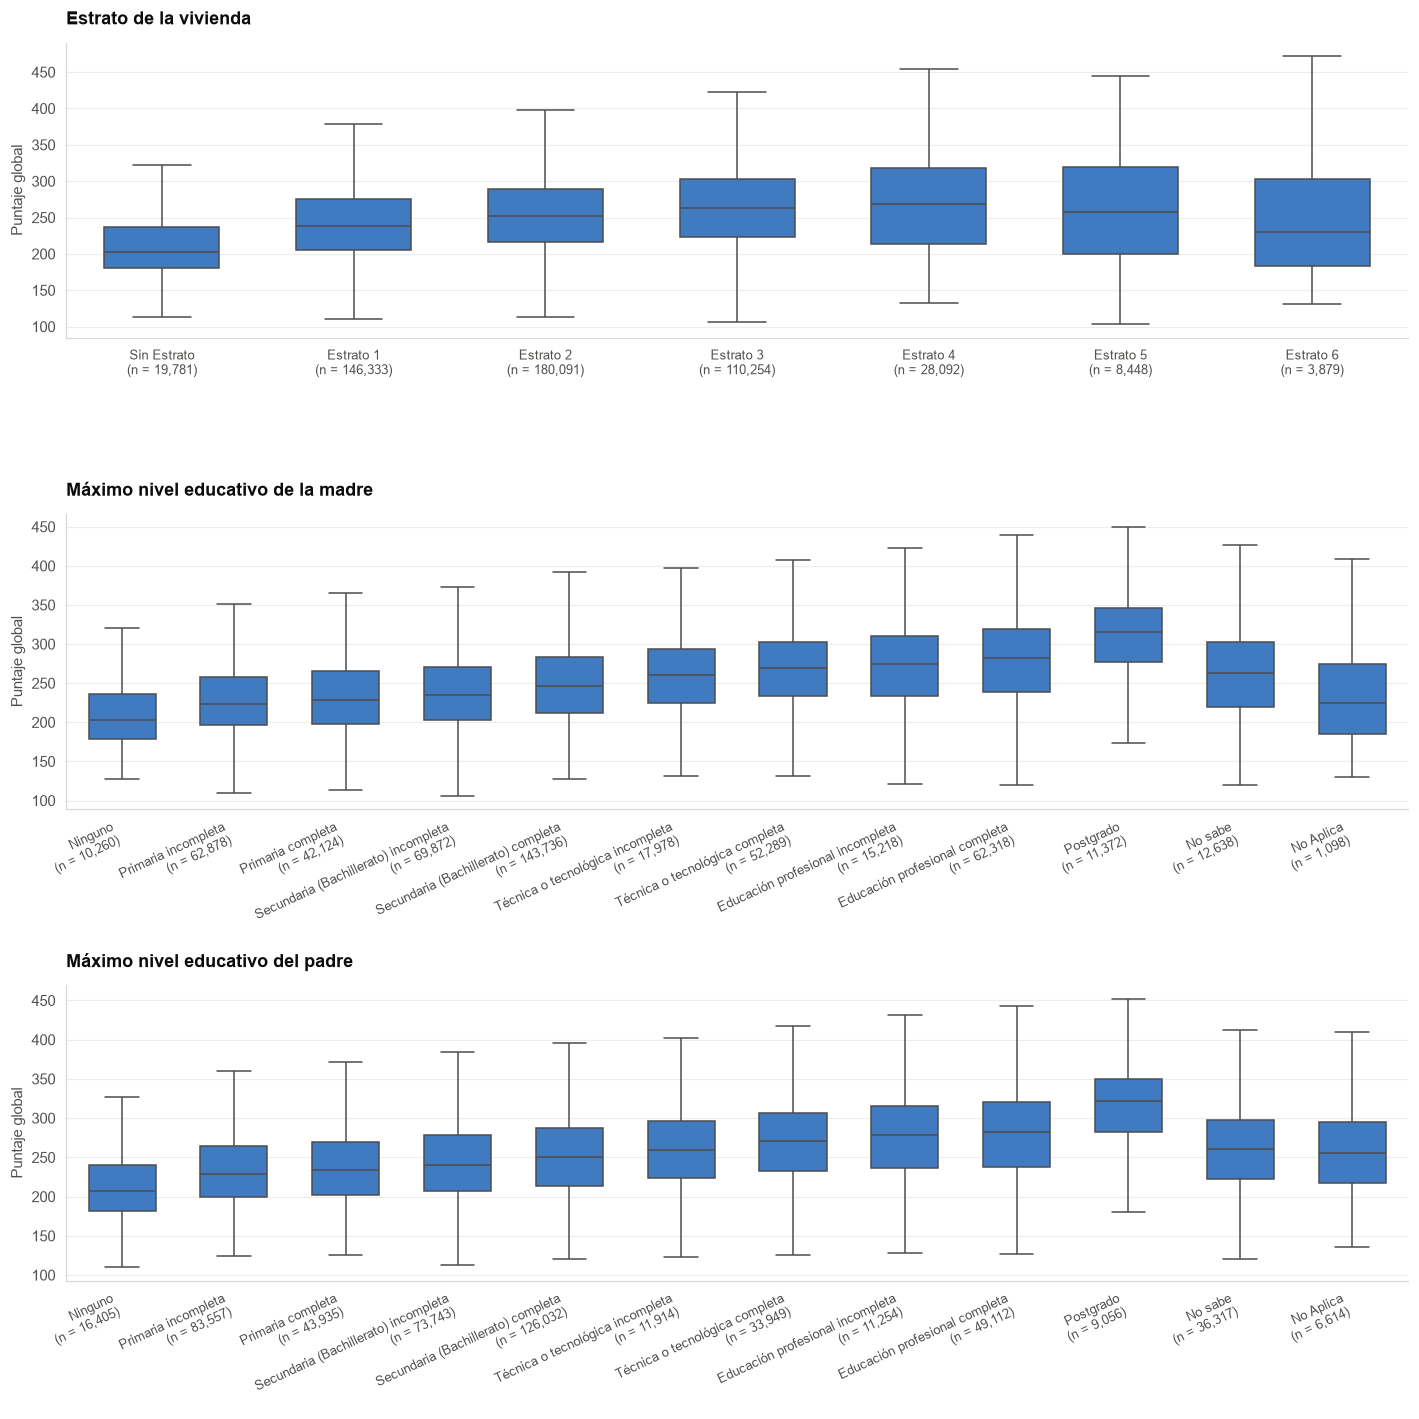
\includegraphics[width=0.78\linewidth]{assets/images/data/family_ordinal.png}
            \captionof{figure}{Puntaje global según estrato de la vivienda y
            máximo nivel educativo de la madre y del padre.}
            \label{family_ordinal}
        \end{strip}

        Tener internet (+31,8 puntos) y computador (+31,7) marcan una diferencia
        muy superior a la del automóvil (+23,6) y la lavadora (+20,8), y en 2022
        todavía el 27\,\% de los hogares declaraba no tener internet. La
        composición del hogar no es monótona (Fig.~\ref{family_binary}): el
        puntaje es máximo en hogares de 3 a 4 personas (257,1) y en viviendas de
        tres cuartos (255,8), y desciende hacia ambos extremos, hasta 225,0 en
        hogares de 9 o más personas y 232,3 en viviendas de seis o más cuartos,
        frecuentes en zonas rurales de bajo ingreso.

        \begin{strip}
            \centering
            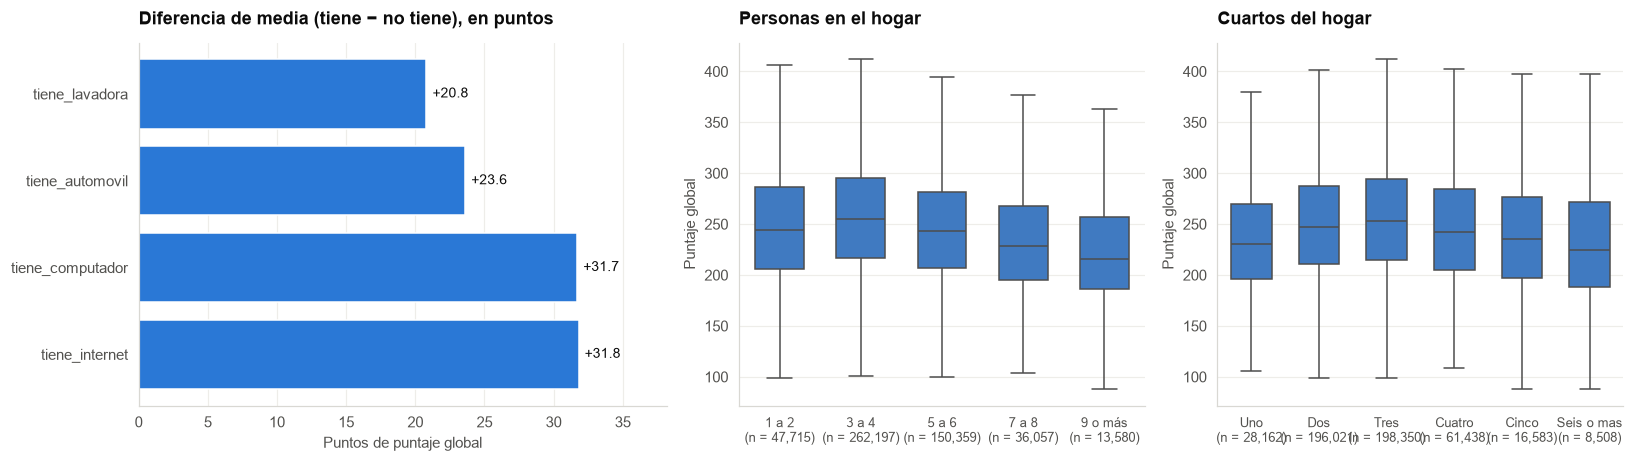
\includegraphics[width=0.98\linewidth]{assets/images/data/family_binary.png}
            \captionof{figure}{Diferencia de puntaje medio según tenencia de
            bienes del hogar, y puntaje según personas y cuartos del hogar.}
            \label{family_binary}
        \end{strip}

    \subsection{Variables del colegio}
        La Tabla~\ref{school_table} y la Fig.~\ref{school_variables} resumen las
        variables del colegio. Los colegios no oficiales promedian 272,6 puntos
        frente a 243,6 de los oficiales (29 puntos), los urbanos 254,6 frente a
        228,4 de los rurales (26,2 puntos), y la jornada es la variable con mayor
        rango: la completa promedia 280,8 mientras que la sabatina (212,7) y la
        nocturna (210,6) quedan 70 puntos por debajo. El carácter académico
        (253,9) supera levemente al técnico (243,3). Contra lo esperado, los
        colegios marcados como bilingües promedian 247,0, por debajo de los no
        bilingües (252,1), lo que sumado a su 18\,\% de faltantes hace del
        indicador una variable poco confiable. Los colegios femeninos (285,5) y
        masculinos (294,2) superan por mucho a los mixtos (249,0), pero son grupos
        pequeños compuestos sobre todo por colegios privados.

        \begin{table}[H]
            \centering
            \caption{Puntaje global medio según variables del colegio}
            \label{school_table}
            \begin{tabular}{|l|r|r|}
                \hline
                \textbf{Variable y nivel} & \textbf{$n$} & \textbf{Media} \\
                \hline
                Naturaleza: Oficial & 412.313 & 243,6 \\
                \hline
                No oficial & 120.478 & 272,6 \\
                \hline
                Área: Urbano & 441.577 & 254,6 \\
                \hline
                Rural & 91.214 & 228,4 \\
                \hline
                Jornada: Completa & 76.897 & 280,8 \\
                \hline
                Única & 146.360 & 252,0 \\
                \hline
                Mañana & 208.530 & 248,2 \\
                \hline
                Tarde & 49.187 & 245,5 \\
                \hline
                Sabatina & 28.116 & 212,7 \\
                \hline
                Noche & 23.701 & 210,6 \\
                \hline
                Carácter: Académico & 269.918 & 253,9 \\
                \hline
                Técnico/académico & 174.947 & 248,9 \\
                \hline
                Técnico & 58.697 & 243,3 \\
                \hline
            \end{tabular}
        \end{table}

        \clearpage
        \begin{strip}
            \centering
            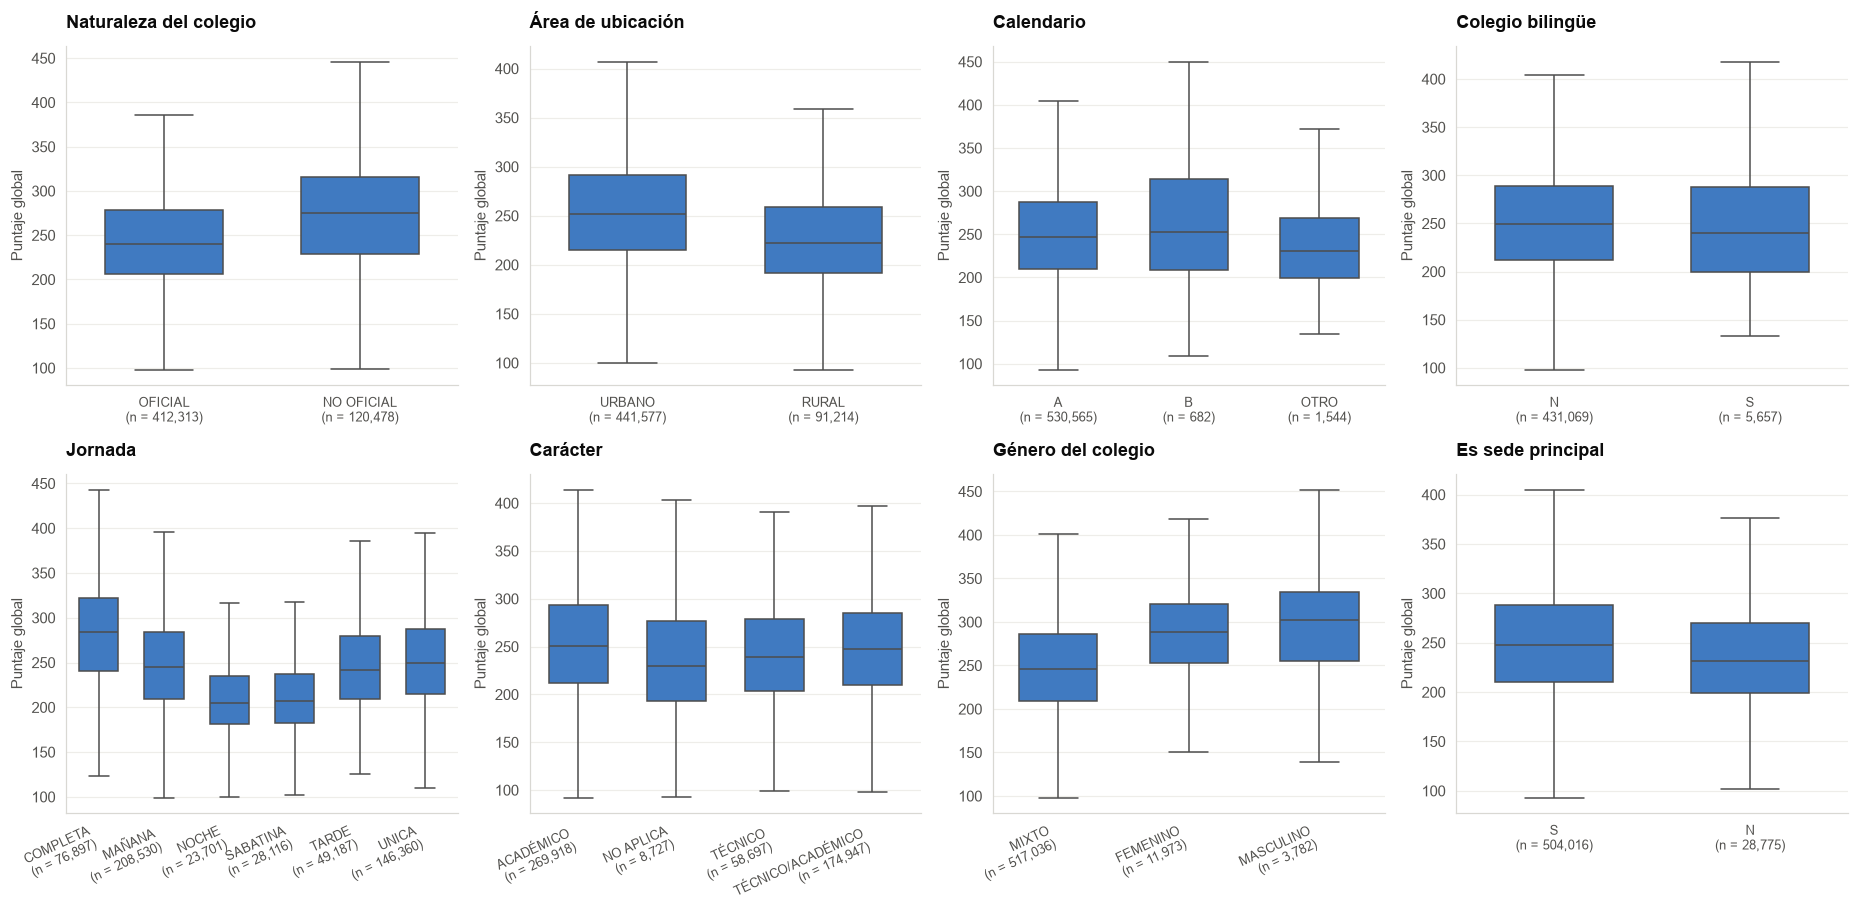
\includegraphics[width=0.98\linewidth]{assets/images/data/school_variables.png}
            \captionof{figure}{Puntaje global según naturaleza, área,
            calendario, bilingüismo, jornada, carácter, género y sede del
            colegio.}
            \label{school_variables}
        \end{strip}

        El cruce entre naturaleza y área (Tabla~\ref{crosstab}) desenreda ambos
        efectos. Entre los colegios oficiales la brecha urbano-rural es de 24
        puntos, pero entre los no oficiales se invierte: los privados rurales,
        pocos y en buena parte colegios campestres, promedian 291,1, el valor más
        alto de las cuatro celdas. Un modelo lineal necesitará un término de
        interacción entre ambas variables.

        \begin{table}[H]
            \centering
            \caption{Puntaje global medio y tamaño según naturaleza y área del colegio}
            \label{crosstab}
            \begin{tabular}{|l|r|r|r|r|}
                \hline
                & \multicolumn{2}{c|}{\textbf{Media}} & \multicolumn{2}{c|}{\textbf{$n$}} \\
                \hline
                \textbf{Naturaleza} & Rural & Urbano & Rural & Urbano \\
                \hline
                No oficial & 291,1 & 271,7 & 5.328 & 115.150 \\
                \hline
                Oficial & 224,5 & 248,6 & 85.886 & 326.427 \\
                \hline
            \end{tabular}
        \end{table}

    \subsection{Variables geográficas}
        La brecha regional es grande y ordenada (Fig.~\ref{geography}). Bogotá
        (270,2), Boyacá (268,6), Santander (267,0) y Cundinamarca (262,8)
        encabezan la lista; Chocó (206,1), Vaupés (213,7), Amazonas (215,5),
        Vichada (217,9) y La Guajira (221,5) la cierran. Entre el primero y el
        último hay 64,1 puntos, más que la diferencia entre colegios oficiales y
        privados, y solo 11 de los 33 departamentos superan la media nacional de
        250,1. Varios departamentos tienen muy pocos estudiantes (Guainía 389,
        Vaupés 434, San Andrés 577), lo que exige una codificación regularizada.

        \begin{figure}[H]
            \centerline{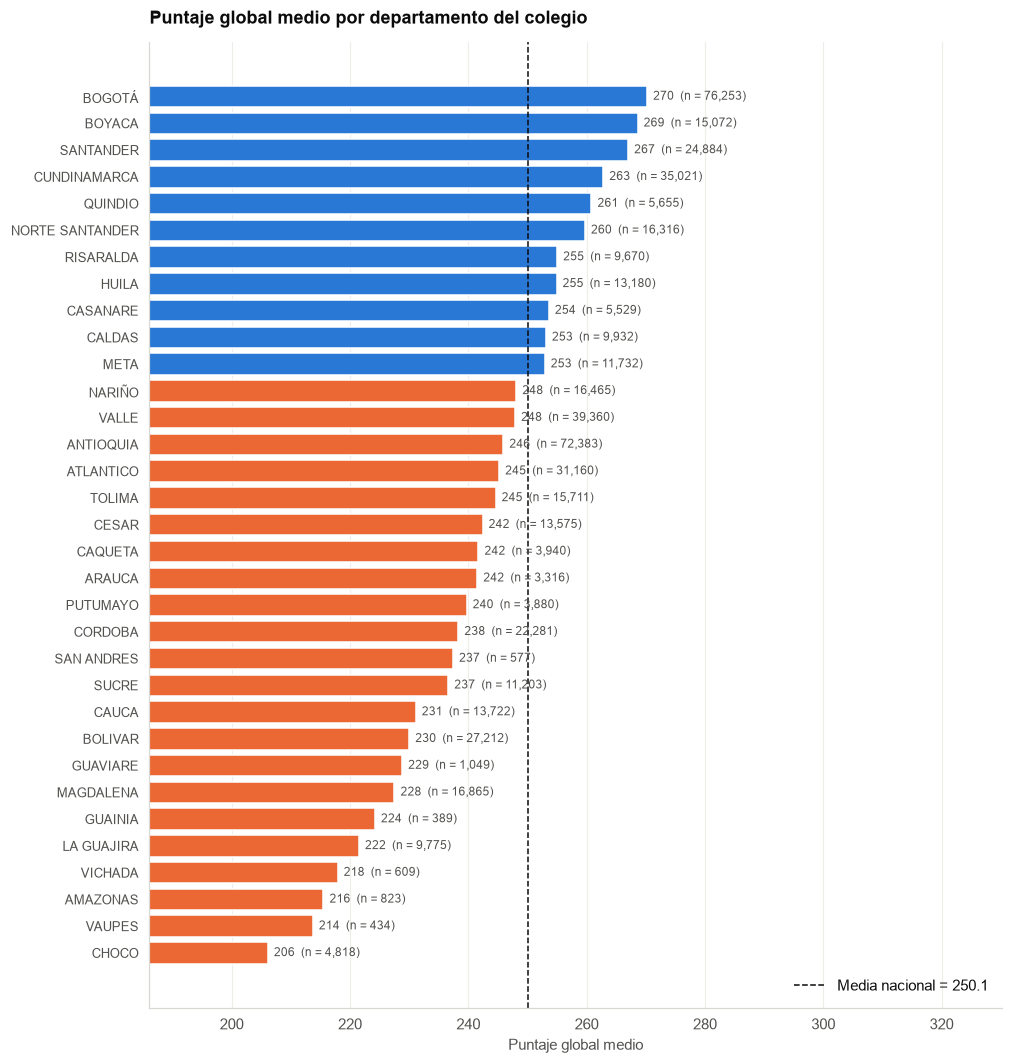
\includegraphics[width=1\linewidth]{assets/images/data/geography.png}}
            \caption{Puntaje global medio por departamento del colegio; en azul
            los departamentos por encima de la media nacional y en naranja los
            que están por debajo.}
            \label{geography}
        \end{figure}

    \subsection{Correlaciones y ajuste lineal exploratorio}
        La matriz de correlación de Spearman (Fig.~\ref{correlation_matrix})
        muestra el contraste buscado, los puntajes por área correlacionan entre
        0,91 y 0,92 con el global mientras que ninguna variable explicativa
        legítima supera 0,35 (Tabla~\ref{spearman_table}). Las variables del hogar
        están además correlacionadas entre sí (educación de la madre y del padre
        0,61; computador e internet 0,48), de modo que miden facetas del mismo
        nivel socioeconómico.

        \begin{table}[H]
            \centering
            \caption{Correlación de Spearman de las variables candidatas con el puntaje global}
            \label{spearman_table}
            \begin{tabular}{|l|r|}
                \hline
                \textbf{Variable} & $\boldsymbol{\rho}$ \\
                \hline
                Educación de la madre & 0,35 \\
                \hline
                Edad & $-$0,32 \\
                \hline
                Educación del padre & 0,32 \\
                \hline
                Tiene computador & 0,30 \\
                \hline
                Tiene internet & 0,28 \\
                \hline
                Colegio no oficial & 0,22 \\
                \hline
                Estrato & 0,19 \\
                \hline
                Colegio urbano & 0,19 \\
                \hline
                Jornada completa o única & 0,19 \\
                \hline
                Tiene automóvil & 0,19 \\
                \hline
                Tiene lavadora & 0,17 \\
                \hline
                Personas en el hogar & $-$0,11 \\
                \hline
                Género femenino & $-$0,07 \\
                \hline
                Colegio bilingüe, cuartos, calendario B & $|\rho| \le 0{,}01$ \\
                \hline
            \end{tabular}
        \end{table}

        \clearpage
        \begin{strip}
            \centering
            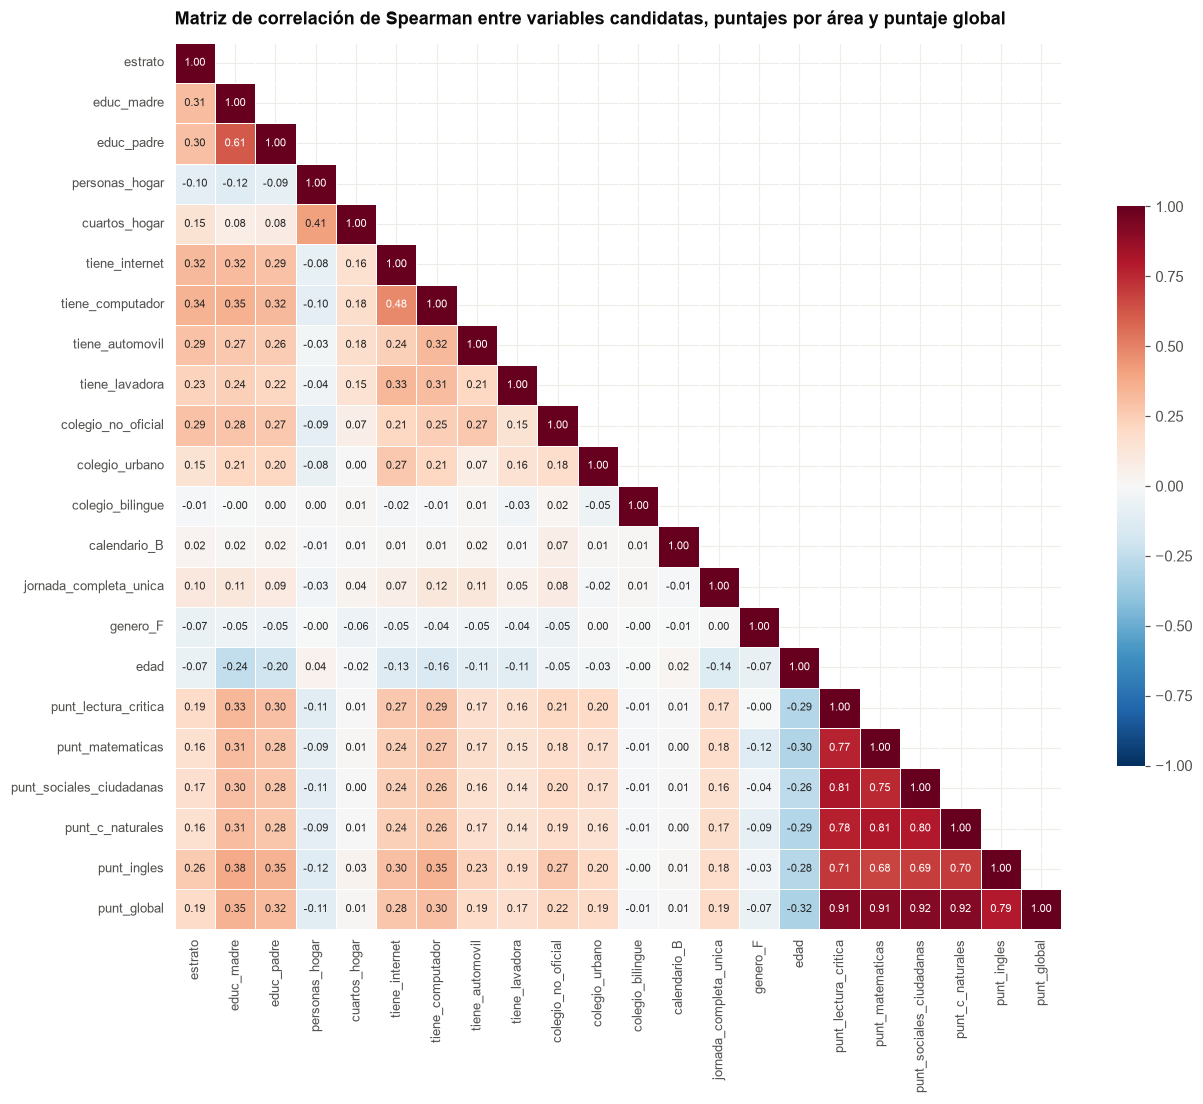
\includegraphics[width=0.72\linewidth]{assets/images/data/correlation_matrix.png}
            \captionof{figure}{Matriz de correlación de Spearman entre las
            variables candidatas codificadas, los puntajes por área y el puntaje
            global.}
            \label{correlation_matrix}
        \end{strip}

        Una regresión lineal sobre las variables codificadas, con 200.000 filas
        completas y partición 80/20, alcanza un $R^2$ de 0,242 y un MAE de 36,5
        puntos frente a 42,6 de predecir siempre la media, una reducción del
        14\,\%. Los coeficientes ratifican los resultados bivariados: colegio no
        oficial (+14,4 puntos), computador (+11,4), jornada completa o única
        (+11,1), internet (+10,1) y colegio urbano (+9,3) son los mayores efectos
        por unidad; cada nivel educativo de la madre suma 3,0 puntos y cada año
        de edad resta 2,9. El estrato queda con un coeficiente casi nulo
        ($-0{,}56$) porque los bienes del hogar y la educación de los padres
        absorben su información.

    \subsection{Hallazgos y decisiones para la fase 2}
        Los hallazgos anteriores se traducen en las decisiones de preparación de
        datos e ingeniería de variables de la Tabla~\ref{decisions}. Con ellas, el
        conjunto de trabajo para la fase 2 queda en 532.792 registros y cerca de
        22 variables explicativas, con el puntaje global como objetivo.

        \clearpage
        \begin{strip}
            \centering
            \captionof{table}{Hallazgos del análisis exploratorio y decisiones para la fase 2}
            \label{decisions}
            \small
            \begin{tabular}{|L{7.6cm}|L{9.6cm}|}
                \hline
                \textbf{Hallazgo} & \textbf{Decisión} \\
                \hline
                Cada registro aparece dos veces & Eliminar duplicados antes de particionar. \\
                \hline
                El global es función exacta de las áreas & Excluir \texttt{punt\_*} por área y \texttt{desemp\_ingles}. \\
                \hline
                La ausencia del cuestionario es informativa (21,5 puntos menos) & Conservar faltantes como categoría \textit{no respondió} e indicador de cuestionario incompleto. \\
                \hline
                Columnas constantes, casi constantes, identificadores y nombres & Descartarlas; conservar departamento y municipio del colegio. \\
                \hline
                Educación de los padres e internet/computador lideran & Educación como ordinal 0 a 9 con \textit{No sabe} como nivel propio; bienes binarios. \\
                \hline
                El estrato se quiebra en 5 y 6 & Probarlo como nominal o agrupar 4 a 6. \\
                \hline
                Personas y cuartos en forma de U & Crear personas por cuarto; tratarlas como categóricas. \\
                \hline
                La edad marca extraedad & Edad numérica e indicador de extraedad; descartar tipo de documento. \\
                \hline
                Jornada, naturaleza y área con interacción & Nominales más interacción naturaleza $\times$ área. \\
                \hline
                Indicador bilingüe poco confiable & Descartarlo o conservarlo con \textit{no reportado}. \\
                \hline
                Brecha regional con departamentos pequeños & \textit{One-hot} o codificación por objetivo suavizada; municipio solo por objetivo. \\
                \hline
                $R^2$ lineal de 0,242 & Referencia: regresión lineal regularizada; meta de la fase 3: superarla con modelos no lineales. \\
                \hline
            \end{tabular}
        \end{strip}

    \section{Conclusiones}
    \begin{itemize}
        \item El conjunto \textit{Resultados únicos Saber 11} del periodo 2022-4
        es apto para el problema planteado, puesto que es público, con licencia
        abierta, tiene una variable objetivo continua y bien comportada (media
        250,1, desviación 51,8, asimetría 0,28) y reúne, para 532.792
        estudiantes, información del hogar, del colegio y de la geografía que
        existe antes de la prueba.

        \item La verificación de calidad fue tan importante como el análisis de
        las variables, dado que la mitad de las filas descargadas eran duplicados
        exactos y el puntaje global resultó ser una función determinista de los
        puntajes por área. Ambos hallazgos, de pasarse por alto, habrían
        producido métricas de modelado ficticias.

        \item Las tres hipótesis de trabajo reciben respaldo preliminar. El nivel
        socioeconómico del hogar, en particular la educación de los padres y el
        acceso a internet y computador, concentra las asociaciones más altas
        (H1); las características del colegio, sobre todo la jornada y la
        naturaleza, aportan brechas propias de 29 a 70 puntos y una interacción
        con el área (H2); y el departamento del colegio introduce una brecha de
        64 puntos entre Bogotá y Chocó que ninguna variable individual explica
        por sí sola (H3).

        \item Ninguna variable aislada correlaciona más de 0,35 con el puntaje y
        una regresión lineal aditiva explica el 24,2\,\% de la varianza con un
        error absoluto medio de 36,5 puntos. Ese es el punto de partida honesto
        del proyecto: el modelo de referencia de la fase 2 deberá reproducirlo
        con la partición definitiva y los modelos de la fase 3 deberán superarlo
        capturando las relaciones no lineales y las interacciones identificadas.

        \item Los valores faltantes no son aleatorios, quienes no responden el
        cuestionario obtienen 21,5 puntos menos, y varias variables ordinales no
        se comportan como tales (estrato, personas y cuartos del hogar). La
        estrategia de preparación debe conservar esa información en lugar de
        imputarla o descartarla, lo que define el plan de limpieza e ingeniería
        de variables de la siguiente actividad.
    \end{itemize}

    \vspace{10pt}

    Como trabajo futuro inmediato, la fase 2 implementará las doce decisiones de
    la Tabla~\ref{decisions}, construirá la partición definitiva en
    entrenamiento, validación y prueba, y establecerá el modelo de referencia; las
    fases 3 y 4 compararán modelos no lineales con ajuste de hiperparámetros,
    interpretarán el modelo final y comunicarán los resultados. Quedan abiertas
    la extensión a varios periodos y el uso de información agregada por colegio y
    municipio como variables de contexto.


    \appendices
    \section{Cuaderno de Google Colab}
    Todo el desarrollo descrito en este informe se implementó en un único
    cuaderno de Google Colab titulado \textit{Predicción del puntaje global de la
    prueba Saber 11 a partir de variables socioeconómicas y del colegio}, que se
    conserva también en el repositorio del proyecto como
    \texttt{notebooks/01\_planteamiento\_y\_eda.ipynb}. Los segmentos de código
    reproducidos en las secciones de metodología y resultados corresponden, uno a
    uno y en el mismo orden, a las celdas de ese cuaderno, y cada uno tiene su
    archivo espejo en \texttt{utils/codes/}.

    \vspace{10pt}

    \begin{tcolorbox}[
        sharp corners,
        colback=green!7!white,
        colframe=green!55!black,
        boxrule=1.2pt,
        fonttitle=\bfseries,
        title=Cuaderno interactivo disponible en Google Colab
    ]
        \centering

        \hypersetup{pdfborder={0 0 0}}
        \urlstyle{same}

        {\color{green!40!black}%
        \url{https://colab.research.google.com/drive/120GLTvDurcx6kycc91pffk8ilKFocwyq?usp=sharing}}

    \end{tcolorbox}

    \vspace{10pt}

    El cuaderno está organizado en doce secciones que siguen el mismo hilo
    argumental del informe:

    \vspace{10pt}

    \begin{itemize}
        \item Planteamiento del problema, pregunta de investigación, objetivos,
        hipótesis y alcance.

        \item Preparación del entorno e identidad gráfica.

        \item Carga y descripción del conjunto de datos, con el diccionario de
        variables.

        \item Estructura y calidad de los datos: duplicados, columnas constantes,
        valores faltantes y conversión de tipos.

        \item La variable objetivo: distribución y verificación de la fórmula del
        puntaje global.

        \item Variables del estudiante.

        \item Variables del hogar.

        \item Variables del colegio.

        \item Variables geográficas.

        \item Correlaciones y ajuste lineal exploratorio.

        \item Hallazgos y decisiones para la fase 2.

        \item Conclusiones.
    \end{itemize}

    \vspace{10pt}

    Su ejecución no requiere ninguna instalación ni descarga manual, puesto que el
    conjunto de datos se obtiene con \textit{kagglehub} desde la copia pública
    publicada en Kaggle \cite{rubiano2026kaggle}, sin necesidad de cuenta, y todas
    las dependencias vienen preinstaladas en el entorno estándar de Colab. La
    descarga del archivo Parquet de 31,5 MB toma unos segundos y el cuaderno
    completo se ejecuta en menos de cinco minutos. La única fuente de aleatoriedad es el
    muestreo del ajuste lineal exploratorio, gobernado por la semilla
    \texttt{RANDOM\_STATE = 42}, de modo que todas las cifras reportadas se
    reproducen exactamente.


    \bibliographystyle{IEEEtran}
    \bibliography{\repo utils/references/references.bib}
\end{document}
